\subsubsection{Smallest measurable torque}
\label{sec:SmallTorque}

\begin{wrapfigure}[7]{R}{0.38\textwidth}
	\centering
	%\vspace{-5pt}
	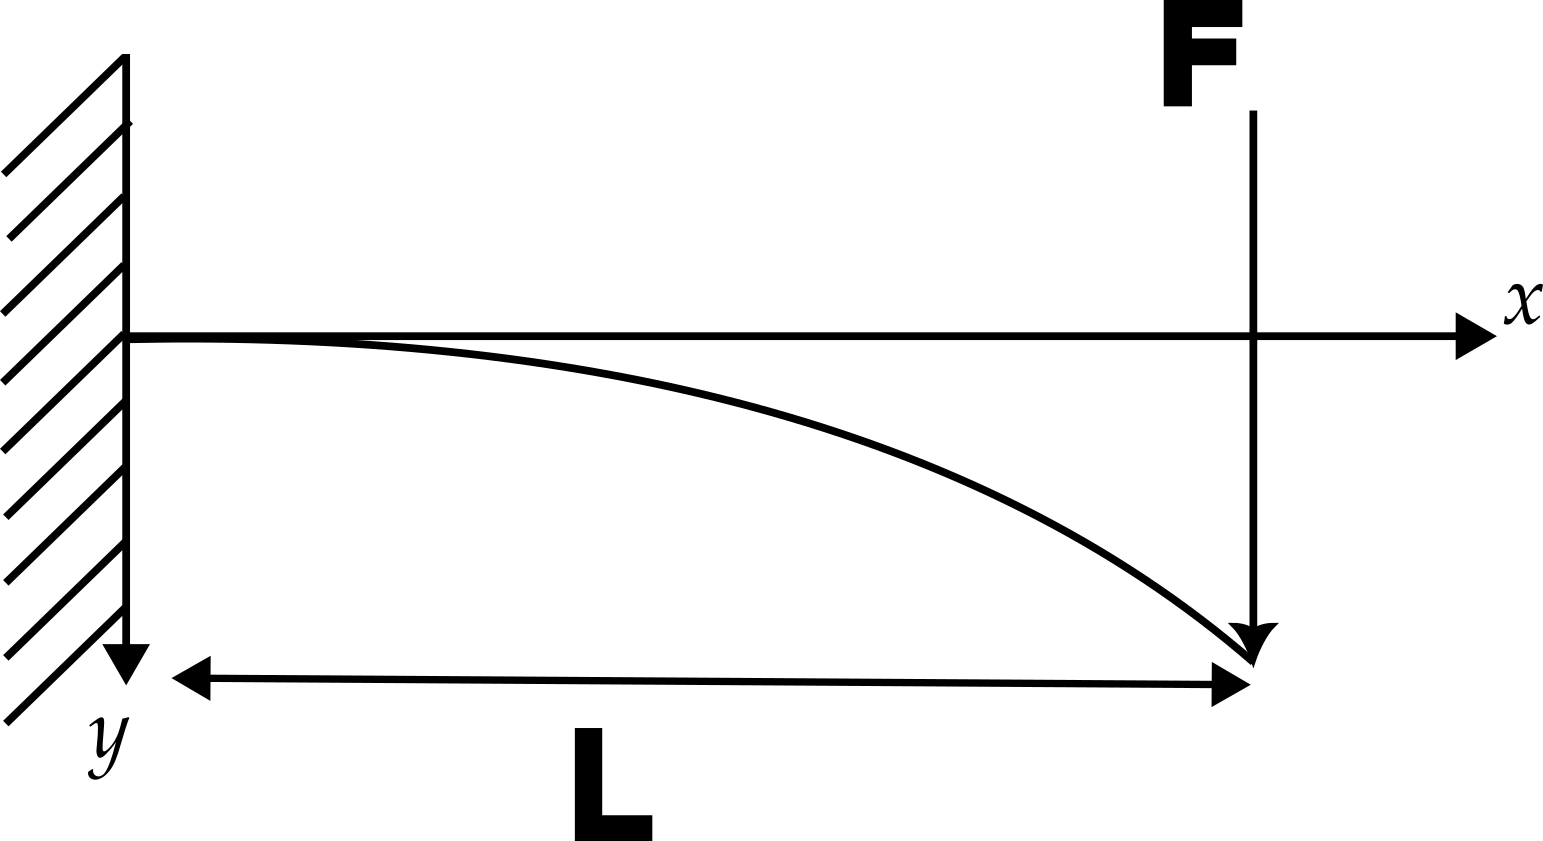
\includegraphics[width=\linewidth]{Assets/cantileverDiagram.png}
	\caption{Cantilever Beam of length L with concentrated load F at the free end.}
	\label{fig:cantileverDiagram}
	%\vspace{10pt}
\end{wrapfigure}

For torque measurements, the sensitivity of cantilever-based torque sensors is determined primarily by the relationship between the applied tip load and the strain induced at the fixed end of the beam. Figure \ref{fig:cantileverDiagram} shows a diagram for a thin cylindrical beam of length $L$ fixed at one end and subjected to a transverse point load $F$ at the free tip. Classical beam theory \cite{hibbeler2016mechanics,Chiu2016CharacterizationOA} gives the maximum surface strain as

\begin{equation}
	\epsilon = \frac{32 F L}{\pi E D^3},
	\label{eq:strain_beam}
\end{equation}

\noindent where $D$ is the diameter, and $E$ is the Young’s modulus. This relationship indicates that the strain is inversely related to the Young's modulus and the cube of the diameter and directly proportional to beam length. As a result, longer and thinner rods increase the observable signal by producing greater strain for the same applied force.  

Following the geometry used by Chiu \textit{et al.} (2016)\cite{Chiu2016CharacterizationOA}, a wire of $L = 69.85\,{mm}$ and $D = 0.64\,{mm}$ fabricated from Nitinol ($E = 66.2\,{GPa}$) achieved an empirical detection limit of $0.49\,{mN}$. Using Equation~\ref{eq:strain_beam}, this translates to a geometric sensitivity factor on the order of $L/D^3 \approx 2.66\times10^8\,{m^{-2}}$, isolating the geometry-dependent amplification of strain and therefore serving as a design metric for mechanical sensitivity. 

A similar configuration can, in principle, achieve micro-Newton sensitivity when paired with a low-noise amplification circuit, provided the strain gauge and readout maintain linear response and the system noise floor remains below the equivalent strain corresponding to the smallest measurable force.

%\subsection{Conversion from Strain to Electrical Signal}

In the actual implementation, a metallic foil strain gauge bonded to the beam surface, which its position is shown in Figure \ref{fig:cantilever3d} and \ref{fig:rods}, converts the mechanical strain into a measurable change in electrical resistance. For small elastic deformations, the fractional change in resistance is linearly related to strain through the gauge factor $G_F$ \cite{fraden2016handbook,MicroMeasurements,OmegaSG},

\begin{equation}
	\frac{\Delta R}{R} = {G_F} \, \epsilon,
	\label{eq:resistance_strain}
\end{equation}

\noindent
where $G_F$ is typically in the range of $2.0$–$2.2$ for constant foil gauges. 
Combining Equations~\ref{eq:strain_beam} and \ref{eq:resistance_strain} gives the total resistance change due to an applied tip force.

\begin{equation}
	\Delta R = R_0 \, {G_F} \, \frac{32 F L}{\pi E D^3}.
	\label{eq:resistance_force}
\end{equation}

\noindent
This resistance change is converted to a differential voltage when the gauge is part of a Wheatstone bridge circuit. For a half-bridge configuration, where two active strain gauges form adjacent arms of the bridge, the small-signal output voltage under excitation $V_{exc}$ is approximately \cite{fraden2016handbook,NI_AN078_1998}

\begin{equation}
	V_{out} \approx \frac{V_{exc}}{2} \, G_F \, \epsilon,
	\label{eq:bridge_output}
\end{equation}

\noindent assuming perfect linearity, little temperature drift, and perfect bridge balancing. The direct proportionality between applied force and bridge voltage may be obtained by combining Equation~\ref{eq:strain_beam} into \ref{eq:bridge_output},

\begin{equation}
	V_{out} = 16 \, G_F \, V_{exc} \frac{L}{\pi E D^3} \, F.
	\label{eq:force_to_voltage}
\end{equation}

In practice, the smallest detectable force is governed by the combined noise of the gauge, bridge, and amplifier system. 
If the noise-equivalent output voltage $V_{noise}$ corresponds to a minimum detectable strain $\epsilon_{min} = \frac{2V_{noise}}{(V_{exc} G_F G)}$, then the force detection limit follows from Equation~\ref{eq:strain_beam} as

\begin{equation}
	F_{min} = \frac{\pi E D^3}{32 L} \, \epsilon_{min}.
	\label{eq:force_limit}
\end{equation}

Theoretically, the sensor can resolve forces in the milli-Newton range by optimizing the geometric ratio $L/D^3$, minimizing circuit noise, and selecting materials with moderate elastic modulus (e.g., aluminum or Nitinol). Using the parameters reported by Chiu \textit{et al.} (2016), such as bridge noise of $\sigma_V = 3$ mV and gain of 100, Equation~\ref{eq:force_limit} yields a minimum detectable force of $F_{\min} = 0.161~$mN (see Appendix~\ref{app:smallestTorque} for sample calculations). This theoretical floor assumes ideal amplification and no parasitic noise; in practice, real circuit noise raises the empirical detection limit, as Chiu et al. report 0.49 mN approximately three times above the theoretical floor of 0.161 mN, consistent with real-world imperfect conditions.

For the present design, the limit of detection is expressed in terms of torque. This is obtained by multiplying the minimum detectable force by the transfer arm length $r$, as described in Sections~\ref{sec:TorqMeasureApp} and \ref{sec:circuitDesignNsensor}. Using the parameters summarized in Table~\ref{tab:sensor_params}, the minimum detectable force is $\approx$ 0.094 mN, corresponding to a torque resolution of $\sigma_{\tau} = 4.70~\mu$N$\cdot$m under ideal conditions. The experimental test results for glass and plastic are reported in Appendix~\ref{app:addRes_senCal} with aluminum results on Section \ref{sec:restorqueLab}, both following the calibration methodology of Section~\ref{sec:sensorCal}.

\begin{table}[hbt!]
	\centering
	\caption{Summary of the sensor and circuit parameters used for force and torque resolution estimation. Values are set for an aluminum-based sensor, paired with the circuit explained in Section \ref{sec:circuitDesignNsensor}}
	\label{tab:sensor_params}
	\begin{tabular}{|l|c|c|}
		\hline
		Parameter & Symbol & Value \\
		\hline
		Young's modulus & $E$ & 68 GPa \\
		Wire diameter & $d$ & 1.6 mm \\
		Beam length & $L$ & 182 mm \\
		\hline
		Bridge noise & $\sigma_V$ & 0.0005 V \\
		Excitation voltage & $V_{\text{exc}}$ & 5 V \\
		Gauge factor & $G_F$ & 2 \\
		Gain & $G$ & 160 \\
		\hline \hline
		Min. Force & $F_min$ & 0.094 mN \\
		Min. Torque & $\tau_min$ & 4.70~$\mu$ N$\cdot$m  \\
		\hline
	\end{tabular}
\end{table}

These restrictions can be decreased by averaging ($\sigma$ scales as $1/\sqrt{N}$), by increasing mechanical leverage (slope grows almost linearly with cantilever length), or by enhancing the bridge/amplifier noise performance. For quasi-static measurements, the limits of detection may be moved from tens of mg into the single-mg or sub-mg range using a combination technique (longer/thinner cantilever + averaging + low-noise amplifier); dynamic measurements will be constrained by bandwidth and 1/f drift.